\documentclass{beamer}


%%%%%%%%%%%%%%%%%%%%%%%%%%%%%%%%%%%%%%%%%%%%%%%%%%%%%%%%%%%%%%
%%%%%%%%%%%%%%%%%%%%%%%%%%%%%%%%%%%%%%%%%%%%%%%%%%%%%%%%%%%%%%
%%%%%%%%%%%%%%%%%%%%%%   Slavko   %%%%%%%%%%%%%%%%%%%%%%%%%%%%
%%%%%%%%%%%%%%%%%%%%%%%%%%%%%%%%%%%%%%%%%%%%%%%%%%%%%%%%%%%%%%
%%%%%%%%%%%%%%%%%%%%%%%%%%%%%%%%%%%%%%%%%%%%%%%%%%%%%%%%%%%%%%
\usepackage[utf8]{inputenc}

\usepackage{verbatim}
\usepackage{url}
%\usepackage{cases}
\usepackage{algorithm}
%\usepackage[cmex10]{amsmath}
\usepackage{alltt}
\usepackage{algorithmic}
%\usepackage[dvipsnames,usenames]{color} 
\usepackage{xcolor}

\renewcommand{\algorithmicrequire}{\textbf{Input:}}
\renewcommand{\algorithmicensure}{\textbf{Output:}}

\usepackage{graphicx}
\graphicspath{{../graphics/}}
%\DeclareGraphicsExtensions{.jpg}

\usepackage[absolute, overlay]{textpos}
\setlength{\TPHorizModule}{30mm}
\setlength{\TPVertModule}{\TPHorizModule}
\textblockorigin{10mm}{10mm}

\newcommand{\secref}[1]{Section~\ref{#1}}
%\newcommand{\appref}[1]{Appendix~\ref{#1}}
\newcommand{\figref}[1]{Fig.~\ref{#1}}
\newcommand{\tblref}[1]{Table~\ref{#1}}
%\newcommand{\eqref}[1]{Eq.~(\ref{#1})}
\newcommand{\algref}[1]{Algorithm~(\ref{#1})}

\newcommand{\TODO}[0]{{\color{BrickRed}\textbf{TODO}}}
\newcommand{\todo}[1]{{\color{BrickRed}\textbf{TODO:} #1}}
\newcommand{\REDO}[1]{{\color{Mahogany}\textbf{REDO:} \textit{#1}}}
\newcommand{\REFS}[0]{{\color{Sepia}\textbf{REFS}}}
\newcommand{\READ}[1]{{\color{Sepia} #1}}
%%%%%%%%%%%%%%%%%%%%%%%%%%%%%%%%%%%%%%%%%%%%%%%%%%%%%%%%%%%%%%
%%%%%%%%%%%%%%%%%%%%%%%%%%%%%%%%%%%%%%%%%%%%%%%%%%%%%%%%%%%%%%
%%%%%%%%%%%%%%%%%%%%%%%%%%%%%%%%%%%%%%%%%%%%%%%%%%%%%%%%%%%%%%
%%%%%%%%%%%%%%%%%%%%%%%%%%%%%%%%%%%%%%%%%%%%%%%%%%%%%%%%%%%%%%
%%%%%%%%%%%%%%%%%%%%%%%%%%%%%%%%%%%%%%%%%%%%%%%%%%%%%%%%%%%%%%

%PRESENTATION DETAILS
\usetheme{CambridgeUS}
\usecolortheme{default}

\title[Programming in Scala] % (optional, only for long titles)
{Programming in Scala}
\subtitle{TECH Talk}
\author{Slavko Žitnik\inst{1,2}}
\institute[Optilab d.o.o \& UL FRI] % (optional)
{
  \inst{1}%
  Optilab d.o.o.\\
  Dunajska cesta 152\\
  SI-1000 Ljubljana
  \and
  \inst{2}%
  University of Ljubljana\\
  Faculty of computer and information science\\
  Tržaška cesta 25\\
  SI-1000 Ljubljana
}
\date{\today}


\begin{document}

\frame{\titlepage}

\section{Agenda}
\begin{frame}
	\frametitle{Agenda}
	\begin{enumerate}
		\item About Scala
		\item Scala performance
		\item Developer tools for Scala
		\item Basic objects
		\item Control structures
		\item Functions and closures
		\item Classes, continued
		\item Collections
		\item XML
	\end{enumerate}
\end{frame}

\begin{frame}
	\frametitle{About Scala}
	\begin{itemize}
		\item Scala - Scalable language
		\item Designed in 2001 by Martin Odesrky, EPFL
		\item First release in late 2003
	\end{itemize}
	\begin{itemize}
		\item Object-oriented language
		\item Functional language (currying, pattern matching, algebraic data types, lazy evaluation, immutability, etc.)
		\item Scripting language
		\item Statically typed
	\end{itemize}
\end{frame}

\begin{frame}
	\frametitle{Why Scala}
	\begin{itemize}
		\item Runs on JVM (.NET support dropped in 2012)
		\item Fully interoperable with Java \& its libraries
		\item Offers lots of syntactic sugars
		\item Reactive programming: Event-driven, Scalable, Resilient, Responsive
		\item ...
	\end{itemize}
\end{frame}

\begin{frame}
	\frametitle{Scala performance}
	\only<1> {
		\begin{figure}[htb]
 			\centering
			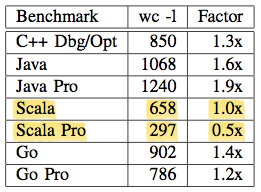
\includegraphics[width=0.5\textwidth]{01_code_lines.png}
			\caption{Number of lines of code.}
		\end{figure}	
	}	
	\only<2> {
		\begin{figure}[htb]
 			\centering
			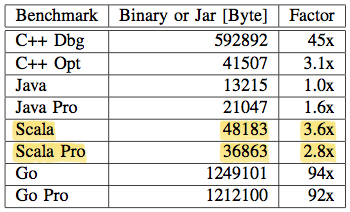
\includegraphics[width=0.6\textwidth]{02_binaries_size.png}
			\caption{Size of compiled binaries.}
		\end{figure}	
	}	
	\only<3> {
		\begin{figure}[htb]
 			\centering
			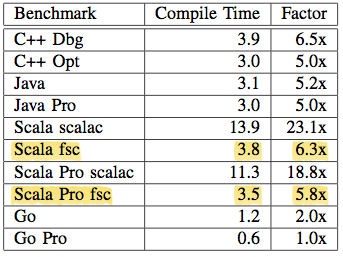
\includegraphics[width=0.6\textwidth]{03_compile_time.png}
			\caption{Time to compile the program.}
		\end{figure}	
	}	
	\only<4> {
		\begin{figure}[htb]
 			\centering
			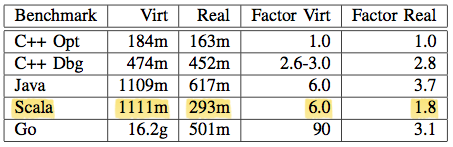
\includegraphics[width=0.6\textwidth]{04_memory_footprint.png}
			\caption{Memory footprint.}
		\end{figure}	
	}	
	\only<5> {
		\begin{figure}[htb]
 			\centering
			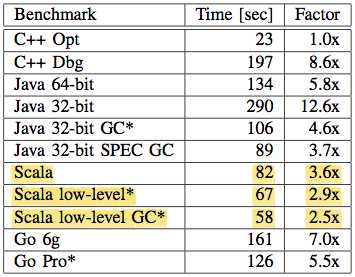
\includegraphics[width=0.6\textwidth]{05_runtime_benchmark.png}
			\caption{Runtime benchmark.}
		\end{figure}	
	}	
		

	Robert Hundt (2011), Loop Recognition in C++/Java/Go/Scala
\end{frame}

\begin{frame}
	\frametitle{IDEs \& REPL}
	\begin{itemize}
		\item Scaladoc
		\item IntelliJIDEA plugin
		\item Eclipse plugin
		\item REPL (Read-Eval-Print-Loop)
		\item SBT (Simple Build Tool)			
	\end{itemize}
	\begin{center}
	{\huge {\bf Console Hands-on}}
	\end{center}
\end{frame}


\section{Hands-on sections}
\begin{frame}
	\frametitle{Basic objects}
	\begin{enumerate}
		\item {\it Rational} class
		\item Override
		\item String formatting
		\item Preconditions
		\item Try-catch block
		\item Auxiliary constructors
		\item Fields
		\item Methods
		\item Implicit conversions
	\end{enumerate}
	\begin{center}
	{\huge {\bf Hands-on}}
	\end{center}
\end{frame}

\begin{frame}
	\frametitle{Control structures}
	\begin{enumerate}
		\item If 
		\item For (nested loops, filters)
		\item While
		\item Break, Continues
	\end{enumerate}
	\begin{center}
	{\huge {\bf Hands-on}}
	\end{center}
\end{frame}

\begin{frame}
	\frametitle{Functions and closures}
	\begin{enumerate}
		\item Functions are first class
		\item Functions are objects
		\item Default parameter values
		\item Partially applied functions
		\item Higher order functions
		\item Currying
	\end{enumerate}
	\begin{center}
	{\huge {\bf Hands-on}}
	\end{center}
\end{frame}

\begin{frame}
	\frametitle{Classes}
	\begin{enumerate}
		\item Trait
		\item Abstract class
		\item Linearization, mix in, hierarchy
		\item Case classes
		\item Pattern matching
	\end{enumerate}
	\begin{center}
	{\huge {\bf Hands-on}}
	\end{center}
\end{frame}

\begin{frame}
	\frametitle{Collections}
	\begin{enumerate}
		\item Mutable, Immutable
		\item Array, List, Set, Map
		\item Option class
		\item Functions: sliding, foldLeft, foldRight,
	dropWhile, filter, mkString, etc.
		\item JavaConversions
	\end{enumerate}
	\begin{center}
	{\huge {\bf Hands-on}}
	\end{center}
\end{frame}

\begin{frame}
	\frametitle{XML}
	\begin{center}
	{\huge {\bf Hands-on}}
	\end{center}
\end{frame}

\section{References}
\subsection{References}
\begin{frame}
	\frametitle{References}
	\begin{itemize}
		\item Coursera class: Functional programming in Scala
		\item Programming in Scala: A Comprehensive Step-by-Step Guide, 2nd Edition by Martin Odersky
		\item Scala in Action by Nilanjan Raychaudhuri (Apr 10, 2013)
		\item Scala for the Impatient by Cay S. Horstmann (Mar 16, 2012)
	\end{itemize}
\end{frame}


\section{Conclusion}
\subsection{Thanks}
\begin{frame}
	\begin{figure}[htb]
   		\centering
   		
\includegraphics[width=1.0\textwidth]{questions.jpg}
	\end{figure}
\end{frame}


\end{document}